\RequirePackage[T1]{fontenc}
\documentclass[conference]{IEEEtran}
\usepackage{amsmath,amssymb,booktabs,graphicx,url,capt-of}
\usepackage[hidelinks]{hyperref}
\setcounter{topnumber}{3}
\setcounter{dbltopnumber}{3}
\renewcommand{\topfraction}{0.92}
\renewcommand{\dbltopfraction}{0.92}
\renewcommand{\textfraction}{0.06}
\renewcommand{\floatpagefraction}{0.8}
\renewcommand{\dblfloatpagefraction}{0.8}
\graphicspath{{../results/controlled_experiment/analysis_v1/}}
% Generated from validated statistics; do not edit numbers manually.
\newcommand{\LegacySuccess}{21.4}
\newcommand{\RewardOnlySuccess}{100.0}
\newcommand{\FixedSuccess}{99.7}
\newcommand{\TerminationSuccess}{0.0}
\newcommand{\PrimaryGain}{78.3}
\newcommand{\CILower}{66.2}
\newcommand{\CIUpper}{89.5}
\newcommand{\RewardOnlyLongSuccess}{100.0}
\newcommand{\FixedLongSuccess}{36.1}
\newcommand{\FixedLongSD}{12.6}
\newcommand{\FixedFeasible}{97.8}
\newcommand{\PDSuccess}{100.0}
\newcommand{\PDLongSuccess}{100.0}
\newcommand{\LegacyTime}{141.2}
\newcommand{\RewardOnlyTime}{50.2}
\newcommand{\FixedTime}{36.5}
\newcommand{\PDTime}{28.6}
\newcommand{\FixedMinusPDTime}{7.9}
\newcommand{\TrainingMinutes}{9.4}

\newcommand{\ind}{\mathbb{1}}
\title{Repairing Mission Rewards for Cellular UAV Control:\\A Factorial Study on a Barcelona Radio Map}
\author{\IEEEauthorblockN{Guillem Moreno Garcia and Evgenii Vinogradov}
\IEEEauthorblockA{Universitat Polit\`ecnica de Catalunya, Barcelona, Spain\\
Research draft, 12 September 2026}}
\begin{document}
\maketitle

\begin{abstract}
A controller can improve communication metrics while failing to complete its
flight. We investigate this failure mode in a documented reimplementation of a
cellular UAV problem using a received Barcelona ray tracing map with 133 base
stations and 17.5 million spatial locations. A four treatment experiment
separates replacement of a binary approach reward from termination on safe
arrival. All treatments share full observations, continuous acceleration,
masked handover actions, and proximal policy optimization. Across five training
seeds and 200 held out routes per seed, the legacy reward achieves
\LegacySuccess\% mission success, reward replacement alone achieves
\RewardOnlySuccess\%, and the combined change achieves \FixedSuccess\%.
Termination alone achieves \TerminationSuccess\%. The combined change improves
success by \PrimaryGain\ percentage points, with a paired 95\% bootstrap
interval of [\CILower, \CIUpper]. On longer routes, reward replacement alone
achieves \RewardOnlyLongSuccess\%, whereas the combined treatment achieves
\FixedLongSuccess\%. A deterministic reference completes all routes in both
sets. The results support repairing the learning objective and show that arrival
termination is not by itself a sufficient remedy. They do not establish
reproduction of the unavailable original simulator, superiority to classical
control, or generalization to other cities.
\end{abstract}

\begin{IEEEkeywords}
UAV, cellular connectivity, reward shaping, handover, reinforcement learning,
mission completion, reproducibility
\end{IEEEkeywords}

\section{Introduction}
A 2026 master's thesis constructed a Barcelona environment using deterministic
ray tracing and real base station locations~\cite[pp.~6--7, Sec.~3.1]{thesis}.
Thesis page locators in this paper refer to printed pages; the PDF viewer page
is two greater. Its reward adds a fixed bonus whenever distance decreases
\cite[p.~12, Eqs.~(13)--(14); p.~15, Table~3]{thesis}, and episodes continue
after arrival to encourage braking~\cite[p.~12, Sec.~5.2]{thesis}.
The thesis reports wandering and prioritization of connectivity over task
completion~\cite[p.~19, Sec.~7.2; p.~21, Sec.~8]{thesis}.
Its listed observation vector omits velocity despite acceleration control
\cite[p.~12, Sec.~5.2; p.~9, Eq.~(2)]{thesis}.
These observations motivate a formulation audit, but the written description
alone cannot identify the behavior of unavailable implementation code.

Cellular UAV control couples motion with network association. A path changes
received powers and cell boundaries, while network decisions change outage,
buffering, and handover costs. Consequently, success requires an explicit
mission definition as well as favorable communication measurements. Related
work studies these objectives jointly, including cargo UAV trajectory planning
and cell association~\cite{cherif}.

The present study asks a narrower, testable question: within a validated shared
environment on the received radio map, does changing the stated reward restore
mission completion, and what additional effect does success termination have?
We use a factorial design rather than simultaneously changing the learning
algorithm and attributing all gains to it. Native hybrid control is an
established approach~\cite{hybrid}; the same hybrid policy and repaired
observation interface are used in every treatment here.

The contribution is an empirical diagnosis with retained artifacts: a source
data audit, a controlled four treatment comparison with five training seeds,
paired evaluations on standard and longer routes, and an explicit deterministic
reference. No new reward shaping theorem or superior general purpose algorithm
is claimed. The original source repository and checkpoints remain unavailable;
this paper therefore reports a reimplementation study, not a reproduction or
an improvement over the thesis's actual trained policy.
Only reward replacement and training termination vary within our factorial
comparison. Other differences from the thesis are shared across all arms and
are not independently ablated. Tables~\ref{tab:modelcomparison} and
\ref{tab:ppocomparison} give the explicit comparison, including unchanged
values and original settings that are not specified.

\section{Data and Shared Environment}
\subsection{Received Radio Map}
The file \texttt{Barcelona\_dataset\_January.h5} contains an
\(133\times5000\times3500\) signed 8 bit RSS array, station identities and
coordinates, operator membership, and transmit powers. Its metadata gives
2.1 GHz, 100 m altitude, and nominal 1 m grid resolution. The file size is
2,327,593,160 bytes. We use the 87 station operator corresponding to the thesis's
first operator~\cite[p.~14, Sec.~6.1]{thesis}. The station counts, frequency,
height, and dimensions match the description~\cite[p.~6, Sec.~3.1.1;
p.~7, Table~2]{thesis}, but exact experiment version identity is not established.

The original stored coordinate vectors span 0--5000 m with 5000 samples and
0--3500 m with 3500 samples. Their spacings are approximately 1.00020004 m and
1.00028580 m. Nearest neighbor lookup uses these vectors; all training and
evaluation use native resolution. Values are promoted to floating point before
radio arithmetic. The untouched source checksum and schema are retained.

A full scan finds that 27.77245\% of all link entries equal $-128$, while the
other entries range from $-110$ to $-25$ dBm. We provisionally interpret $-128$
as an absent usable path and assign it zero received power. The generator's
sentinel and quantization conventions still require confirmation. For the
selected operator, every grid position has at least 38 stations above
$-96$ dBm, and the strongest RSS ranges from $-51$ to $-25$ dBm. Thus the stored
map has no inevitable geographic coverage hole under this RSS threshold.
This observation does not guarantee a permissible handover or adequate SINR.

\subsection{Motion, Mission, and Observations}
The thesis writes scalar speed and a selected direction in its position update
\cite[p.~9, Sec.~3.2, Eq.~(2)]{thesis}. Our shared benchmark instead preserves
an inertial velocity vector at constant altitude. With velocity projection,
\begin{align}
\mathbf v_{t+1}&=\Pi_{\|\mathbf v\|\leq v_{\max}}
 (\mathbf v_t+\mathbf a_t\Delta t),\\
\mathbf p_{t+1}&=\mathbf p_t+
 \tfrac12(\mathbf v_t+\mathbf v_{t+1})\Delta t.
\end{align}
The policy supplies radial and lateral acceleration components in a frame
aligned with the current destination bearing. Their norm is limited to
5 m/s$^2$, and speed is limited to 25 m/s. This continuous action interface
replaces the five acceleration bins and eight headings
\cite[p.~12, Sec.~5.2; p.~15, Table~3]{thesis}. The thesis uses a 100 m/s
penalty threshold~\cite[p.~15, Table~3]{thesis}; ours is a hard 25 m/s cap.
The step is 1 s and the deadline is 200 s. The source gives 1 ms in prose
\cite[p.~14, Sec.~6.1]{thesis} and 0.1 s in Table~3
\cite[p.~15]{thesis}; we explicitly choose a new time discretization.

Safe arrival is the common event
\begin{equation}
\mathcal G_t=\{\|\mathbf p_t-\mathbf g\|\leq10\ \mathrm m,
                  \ \|\mathbf v_t\|\leq2\ \mathrm{m/s}\}.
\end{equation}
The 10 m position tolerance is retained from Table~3~\cite[p.~15]{thesis};
the numerical 2 m/s terminal speed test is our addition to the stated stopping
intention~\cite[p.~9, Sec.~3.2]{thesis}. A boundary crossing, battery exhaustion,
or five consecutive RSS outage samples ends a failure. The thesis explicitly
terminates on energy exhaustion and penalizes boundary, RSS, and speed
violations~\cite[p.~12, Sec.~5.2, Eq.~(14)]{thesis}; our boundary and repeated
outage terminations are additional rules. Speed is constrained directly.
Building geometry supports propagation in the thesis~\cite[p.~6, Sec.~3.1.1]{thesis}.
Our received RSS array does not provide a collision model, and obstacle safety
is outside the evaluated model; we do not assume the original code enforced it.

Every treatment receives the same 42 dimensional observation: position;
destination bearing and distance; radial, lateral, and total velocity;
remaining time encoded by elapsed time; energy; buffer; prior arrival flag;
resource and load phases; network decision phase; serving SINR; outage count;
and candidate RSS, relative positions, identities, and masks. This replaces
the listed six component vector of position, serving station, resource group,
energy, and buffer~\cite[p.~12, Sec.~5.2]{thesis}. Observation repair is shared,
and its independent effect is not estimated.

\subsection{Association and Communication Proxies}
A categorical policy selects stay or one of the four strongest candidate
stations. A request is admissible when candidate RSS exceeds both $-96$ dBm
and serving RSS plus 3 dB. Network actions occur every five seconds, with an
additional opportunity on an observed serving RSS outage. This emergency rule
was introduced during validation, before training, when a periodic decision
could otherwise arrive after the outage failure deadline. We do not implement
or claim a complete 3GPP time to trigger procedure. Masking follows the standard
practice of excluding invalid categorical actions~\cite{masking}.
The inequality follows the thesis's A3 equation~\cite[p.~9, Eq.~(3)]{thesis},
with the numerical offset from Table~3~\cite[p.~15]{thesis}; the five action
candidates and decision interval are our choices. The source greedy controller
uses viability counters~\cite[pp.~13--14, Sec.~5.4]{thesis}, which we do not copy.

There are twelve resource groups and six occupied background groups per
station in a fixed spatial pattern. A shared first available allocation rule
chooses the resource group; resource allocation is not learned. Scenario phase
rotates group labels globally and does not supply independent traffic dynamics.
The source permits learned RBG requests~\cite[p.~9, Sec.~3.3.1;
p.~12, Sec.~5.2]{thesis} and describes random occupancy of at least half the
groups~\cite[p.~14, Sec.~6.1]{thesis}; both differ from our shared allocator.
Since the source RSS is a downlink budget~\cite[p.~7, Eq.~(1)]{thesis}, station powers
are aggregated as a downlink interference proxy:
\begin{equation}
P_k=10^{(\mathrm{RSS}_k-30)/10},\quad
\mathrm{SINR}=\frac{P_s}{N+\sum_{k\ne s}o_kP_k}.
\end{equation}
Here powers are in watts, $o_k$ indicates background occupancy of the selected
group, and noise including the noise figure is $-103.41$ dBm. The ideal service
rate is $1.44\cdot10^6\log_2(1+\mathrm{SINR})$ bit/s. It is neither measured
throughput nor a validated uplink interference model.
This replaces the printed bandwidth-plus-logarithm rate, SNR in dB, and sum of
RSS values labeled uplink interference~\cite[p.~10, Eqs.~(7)--(9)]{thesis}.
It changes the interference model as well as correcting power arithmetic;
we cannot establish whether the original code used the printed expressions.

Deterministic offered traffic is 200 kbit/s, buffer capacity is 1.28 Mbit, and a
handover adds 4800 bits. The control overhead and nominal buffer capacity follow
Table~3~\cite[p.~15]{thesis}, interpreting KB as decimal kilobytes.
Deterministic traffic replaces the Poisson formulation
\cite[pp.~9--10, Eqs.~(5)--(6)]{thesis}; the thesis also gives different data
packet sizes in prose and table~\cite[pp.~14--15, Sec.~6.1, Table~3]{thesis}.
The backlog/service delay retains the ratio in Eq.~(4)~\cite[p.~9]{thesis},
but we explicitly use postservice backlog and censor at 200 s.
Energy is the integral
of $100+0.4\|\mathbf v\|^2$ watts against a 100 kJ budget. This explicit proxy
replaces the mass, efficiency, lift-to-drag and electronics expression
\cite[p.~10, Eq.~(10)]{thesis} and the capacity labeled 1000 kW
\cite[p.~15, Table~3]{thesis}. It does not claim a calibrated rotorcraft model.
Table~\ref{tab:changes}
summarizes the main departures from the source description.

\begin{table}[t]
\caption{Shared reimplementation choices, held fixed across treatments}
\label{tab:changes}\centering\footnotesize
\begin{tabular}{@{}p{.29\columnwidth}p{.64\columnwidth}@{}}
\toprule
Aspect & Declared benchmark choice\\\midrule
Observations & Goal and velocity observed; 42 dimensions\\
Motion & Continuous acceleration, 1 s steps, 25 m/s cap\\
Network & Stay plus four candidates; masks; outage requests\\
Resources & Common deterministic first available allocator\\
Interference & Linear downlink cochannel power proxy\\
Traffic and energy & Deterministic traffic; explicit energy proxy\\
Source equivalence & Original code and checkpoints unavailable\\\bottomrule
\end{tabular}
\end{table}

\section{Reward Treatments and Learning}
\subsection{Why the Binary Approach Bonus Is Suspect}
Let $d_t$ be destination distance, $D_t$ the declared delay proxy, $I_t$ the
linear interference proxy, and $h_t$ a handover indicator. The legacy reward
treatment implements the structure in Eqs.~(13)--(14)
\cite[p.~12]{thesis}, with the equal-policy weights, scales, and bonus in
Table~3~\cite[p.~15]{thesis}:
\begin{align}
r_t^L={}&\frac{.35}{1+10D_t}+\frac{.30}{1+10^5I_t}
       +\frac{.35}{1+100h_t} \nonumber\\
       &+12\ind[d_{t+1}<d_t]-10O_t-10B_t,
\end{align}
where $O_t$ and $B_t$ mark RSS outage and a boundary crossing. Energy exhaustion
overrides the reward with $-10$. The shared speed constraint replaces a soft
speed penalty. The interference input is corrected to watts for all treatments;
thus this is an ablation of the written incentive, not literal replication of
potentially erroneous source equations.

The approach term depends on the sign of progress but not its magnitude. A
controller can receive the same bonus for very slow progress as for efficient
flight. A retreat carries no matching distance cost, permitting positive
approach bonuses on a closed excursion outside the destination region.
Moreover, stopping the episode without a compensating mission objective can
remove future positive reward and reinforce avoidance of completion. Similar
failures motivate potential based shaping~\cite{shaping}.

\subsection{Mission Reward and Terminal Potential}
Define the potential, with $L=100$ m,
\begin{equation}
\Phi(s)=-\frac{d+\|\mathbf v\|^2/(2a_{\max})}{L}.
\end{equation}
The speed term is a stopping distance scale. The replacement reward is
\begin{align}
r_t^M={}&20A_t-20F_t-0.05-0.05c_t \nonumber\\
        &+\gamma\Phi(s_{t+1})-\Phi(s_t),
\end{align}
where $A_t$ marks first safe arrival, $F_t$ a terminal failure before any safe
arrival, and $c_t=\min(D_t,1)+O_t+h_t$. The prior arrival flag is observed, and
the success bonus is paid only once even if training continues afterward.
Set the potential to zero at every terminal, including the deadline. For any
episode ending at $T$, the shaping contribution satisfies
\begin{equation}
\sum_{t=0}^{T-1}\gamma^t
 [\gamma\Phi(s_{t+1})-\Phi(s_t)]=-\Phi(s_0).
\end{equation}
Consequently, within each fixed terminal formulation, shaping preserves the
discounted base objective~\cite{shaping}. This identity is checked numerically.
It does not imply that the finite weighted base reward certifies every physical
constraint or guarantees successful learning.
The identity concerns raw rewards. Running normalization and clipping in PPO
can change the effective update objective; this experiment tests the declared
learning recipe without isolating those interactions.

\begin{table}[t]
\caption{Factorial training treatments}
\label{tab:arms}\centering\footnotesize
\begin{tabular}{lll}\toprule
Label & Reward & Terminate on arrival\\\midrule
Legacy & $r^L$ & No\\
Termination only & $r^L$ & Yes\\
Reward only & $r^M$ & No\\
Both & $r^M$ & Yes\\\bottomrule
\end{tabular}
\end{table}

\begin{figure}[!t]
\centering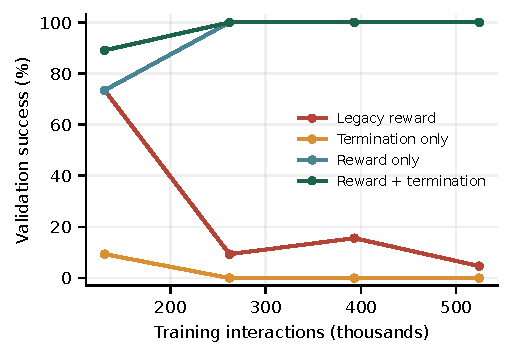
\includegraphics[width=.98\columnwidth]{pilot_learning.pdf}
\caption{Pilot seed 42 on 64 validation routes. Curves are used to document
development and budget choice, not to substitute for the frozen test comparison.}
\label{fig:pilot}
\end{figure}

\subsection{Common PPO Implementation}
All arms use proximal policy optimization~\cite{ppo} with separate actor and
critic networks, each containing two 64 unit tanh layers. The actor has a
Gaussian motion head and a masked categorical association head. Motion samples
are transformed through tanh and the acceleration norm limit; likelihood ratios
are consistently computed in latent action space. The entropy regularizer sums
latent Gaussian and masked categorical entropy.

Training uses 64 parallel lanes, 128 step rollouts, four epochs per rollout,
512 sample minibatches, Adam learning rate $3\cdot10^{-4}$, clip 0.2,
$\gamma=0.99$, GAE parameter 0.95, entropy coefficient 0.005, value coefficient
0.5, and gradient norm limit 0.5. Rewards are divided by a running standard
deviation of discounted returns without subtracting a mean, and clipped to
$[-10,10]$, consistently across arms. Finite horizon terminals are not
bootstrapped. No pretrained model, demonstrations, or imitation loss is used.
The thesis uses Stable Baselines~\cite[p.~13, Sec.~5.3]{thesis}; our PPO is a
new native implementation. Table~\ref{tab:ppocomparison} contrasts every
reported source setting with ours~\cite[p.~16, Table~4]{thesis}.
For example, learning rate increases from $3\cdot10^{-5}$ to $3\cdot10^{-4}$,
entropy weight decreases from 0.01 to 0.005, and the source's 0.03 target KL
is replaced by diagnostic KL logging without an early stopping threshold.

\begin{table*}[t]
\caption{Frozen results: percentages are mean $\pm$ standard deviation over five training seeds. Standard routes are 200--1000 m; longer routes are 1000--1800 m. Each learned policy evaluates 200 routes per split.}
\label{tab:results}\centering\footnotesize
\begin{tabular}{lcccccc}\toprule
 & \multicolumn{2}{c}{Mission success (\%)} & \multicolumn{2}{c}{Recorded feasible success (\%)} & \multicolumn{2}{c}{Successful episodes}\\
Treatment & Standard & Longer & Standard & Longer & Standard & Longer\\\midrule
Legacy & $21.4\pm14.3$ & $0.0\pm0.0$ & $20.8\pm13.9$ & $0.0\pm0.0$ & 214/1000 & 0/1000 \\
Termination only & $0.0\pm0.0$ & $0.0\pm0.0$ & $0.0\pm0.0$ & $0.0\pm0.0$ & 0/1000 & 0/1000 \\
Reward only & $100.0\pm0.0$ & $100.0\pm0.0$ & $98.7\pm1.4$ & $96.0\pm1.1$ & 1000/1000 & 1000/1000 \\
Both & $99.7\pm0.7$ & $36.1\pm12.6$ & $97.8\pm0.8$ & $35.2\pm12.6$ & 997/1000 & 361/1000 \\
Deterministic reference & 100.0 & 100.0 & 97.0 & 95.5 & 200/200 & 200/200 \\
\bottomrule\end{tabular}
\end{table*}


\begin{figure*}[!t]
\centering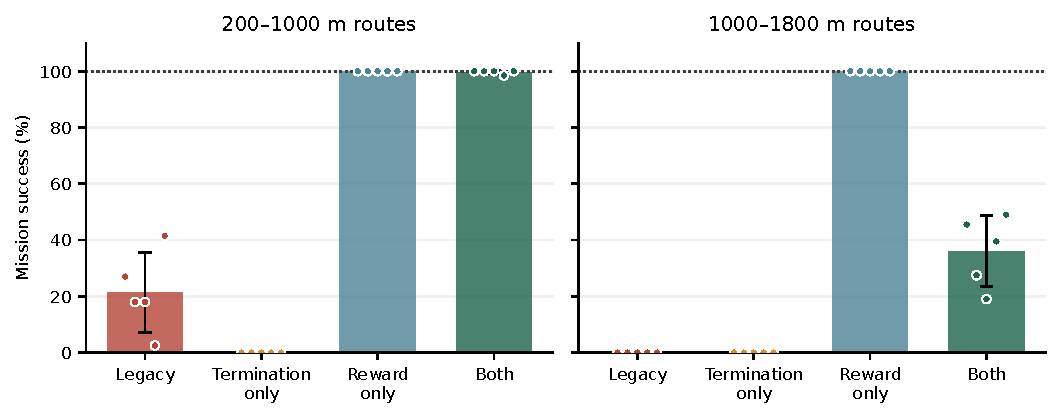
\includegraphics[width=.97\textwidth]{success_comparison.pdf}
\caption{Frozen test mission success. Each dot is one training seed, bars show
the mean, and error bars show seed standard deviation. There are 200 shared
routes per split and five seeds per learned treatment. The dotted line is the
deterministic reference. No test outcome was used to tune the frozen policies.}
\label{fig:success}
\end{figure*}

\section{Evaluation Protocol}
\subsection{Validation, Freeze, and Held Out Routes}
Training uses 4096 routes sampled with lengths 200--1000 m, with 64 separate
validation routes. The final standard set contains 200 new routes of the same
length range. A second set contains 200 routes of length 1000--1800 m. These
are unseen coordinate pairs in the same city, not independent cities or held
out geographic regions. Starts and destinations stay inside documented map
margins. All coordinates, seeds, and background phases are saved.
The original tuning and comparison sections do not specify three independent
training, validation, and test route sets~\cite[pp.~15--16, Secs.~6.2--6.3]{thesis}.
This is a limit of the written protocol, not proof that its unavailable code
lacked such a separation.

Six pilots, using seeds 41 and 42, established learning behavior and the
524,288 interaction budget. All final arms use seeds 1101--1105 and exactly
that budget, totaling 10,485,760 interactions. Source hashes and configuration
were frozen before trained policy test evaluation. The initial feasibility
inspection used separate exploratory route sets, which were retired before
training; final route seeds are 42012 and 42013. Final checkpoints are evaluated
without early stopping or test based selection. Each lane follows the same
ordered training scenario stream across treatments, although successful
termination changes how many episodes fit in an equal interaction budget.

The evaluated continuous action is the Gaussian mean after transformation, and
the network action is the masked categorical mode. Every policy's evaluation
stops at first safe arrival, independently of its training termination rule.
Thus the continuing training treatment is still evaluated as a finite mission.

\subsection{Metrics, Reference, and Uncertainty}
Mission success is primary. Recorded feasible success additionally requires
no packet overflow and an RSS outage fraction at most 5\%. This limited
feasibility label does not imply obstacle or airframe certification. Failure
counts and final distances are retained. Time, path, energy proxy, delay,
interference, SINR, and handovers are reported conditional on success with
their sample counts, avoiding aggregation of failed flights into radio gains.

The deterministic reference points its desired velocity toward the goal, uses
a braking schedule based on stopping distance, and requests the strongest
admissible station. It shares every environmental constraint and resource rule.
It establishes that the tested missions are attainable and provides a practical
nonlearning comparison; it is not asserted to be globally optimal.

We show all five seed outcomes and standard deviations. The primary contrast
is both changes minus legacy success on standard routes. A 10,000 draw crossed
bootstrap resamples the five seed identities and 200 route identities, using
the same sampled identities for both arms. This preserves pairing and avoids
counting 1000 episodes as 1000 independent training runs. Other factorial and
longer route contrasts are secondary. Interval reporting follows the broader
need to expose uncertainty in few run RL evaluations~\cite{statistics}.
Five seeds still provide limited resolution and uncertain tail behavior.

The prespecified practical gate for a positive repair finding requires at least
90\% mean standard mission success, at least 90\% recorded feasible success,
and a positive lower 95\% bootstrap bound for the primary contrast. It is a
reporting gate rather than a claim of statistical or deployment certification.

\begin{figure*}[!t]
\centering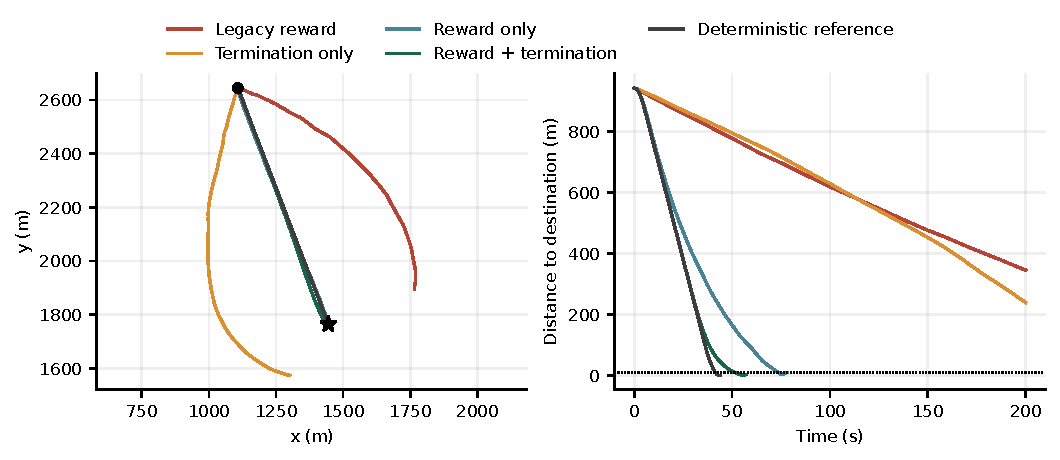
\includegraphics[width=.97\textwidth]{example_trajectory.pdf}
\caption{First standard test route and first declared training seed. The black
circle and star denote start and destination. All learned treatments and the
deterministic reference share the scenario. The dotted distance line marks
10 m; low speed is also required for success.}
\label{fig:trajectory}
\end{figure*}

\begin{table*}[t]
\caption{Standard route metrics conditional on mission success, pooled across the five seeds. The deterministic reference has one run on 200 routes. Different successful subsets prevent unqualified secondary dominance claims. Energy, delay, and interference are the declared proxies.}
\label{tab:metrics}\centering\footnotesize
\begin{tabular}{lrrrrrrrr}\toprule
Treatment & $n$ & Time (s) & Energy (kJ) & Handovers & SINR (dB) & Delay (s) & Outage (s) & Interf. ($\mu$W)\\\midrule
Legacy & 214 & 141.25 & 14.80 & 8.83 & -6.34 & 0.88 & 0.07 & 0.70 \\
Termination only & 0 & n/a & n/a & n/a & n/a & n/a & n/a & n/a \\
Reward only & 1000 & 50.23 & 8.29 & 3.96 & -7.91 & 2.58 & 0.09 & 0.74 \\
Both & 997 & 36.52 & 8.17 & 2.99 & -8.13 & 2.83 & 0.09 & 0.74 \\
Deterministic reference & 200 & 28.62 & 7.99 & 2.38 & -8.51 & 3.45 & 0.09 & 0.74 \\
\bottomrule\end{tabular}
\end{table*}


\section{Results}
\subsection{Completion and Factorial Effects}
Table~\ref{tab:results} and Fig.~\ref{fig:success} present the full frozen
comparison. Reward replacement alone achieves \RewardOnlySuccess\% standard
success compared with \LegacySuccess\% for the legacy reward. The combined
change achieves \FixedSuccess\%, while termination alone achieves
\TerminationSuccess\%. The primary gain is \PrimaryGain\ percentage points,
with a paired bootstrap interval [\CILower, \CIUpper]. Recorded feasible
success for the combined change is \FixedFeasible\%, satisfying the practical
gate. These results identify the replacement reward as the essential tested
intervention; changing arrival termination alone does not resolve the failure.




The pilots also illustrate why longer training cannot automatically repair a
misaligned objective. In pilot seed 42, legacy validation success initially
rises to 73.4\% and then falls to 4.7\% by the final budget. Reward replacement
reaches 100\% by approximately 262,144 interactions and retains it through
the pilot's final checkpoint. Figure~\ref{fig:pilot} is explicitly exploratory
validation evidence from one pilot, not a confidence interval over final seeds.



\subsection{Longer Routes and the Role of Termination}
Reward replacement with continuing training reaches \RewardOnlyLongSuccess\%
success on longer routes. The combined treatment reaches
\FixedLongSuccess\% with seed standard deviation \FixedLongSD\ percentage
points. Thus the treatment that provides efficient completion within the
training range does not necessarily generalize best to longer flights.
Training termination changes episode exposure and visitation distribution even
under equal interaction budgets, but the experiment does not isolate the
mechanism causing this extrapolation difference. The longer route weakness is
retained rather than removed by further test driven tuning.

Figure~\ref{fig:trajectory} shows the first predefined standard test route for
seed 1101, selected by index rather than performance. Its trajectories and
distance traces illustrate the different learned behavior, while the aggregate
tables remain the basis for the conclusions. Proximity by itself is insufficient:
the evaluated success criterion also requires low speed.



\subsection{Efficiency and the Deterministic Reference}
The deterministic reference achieves \PDSuccess\% standard and
\PDLongSuccess\% longer route success. Among successful standard missions,
mean flight times are \LegacyTime\ s for legacy, \RewardOnlyTime\ s for
reward only, \FixedTime\ s for both changes, and \PDTime\ s for the reference.
Because the successful subsets differ, these means alone are not paired
efficiency comparisons. On matched successful standard routes, the combined
policy takes \FixedMinusPDTime\ s more time than the reference on average.
The evidence establishes repair of a learned objective, not an advantage over
the deterministic controller.


Table~\ref{tab:metrics} reports success conditional secondary metrics with
sample counts. The radio summaries are downlink proxies and the energy measure
is uncalibrated. A controller with lower interference or delay on a subset of
completed short routes is not ranked above a controller that completes the
whole route set. Raw per episode records permit matched subset analysis without
concealing failures or mixing physical units.
The original results emphasize SNR, outage, interference, remaining energy,
and handover count~\cite[pp.~16--20, Sec.~7, Figs.~5--8]{thesis}.
Our success rate, terminal speed and distance checks, success conditional
reporting, and paired seed uncertainty are additional evaluation choices.

\section{Validity and Reproducibility}
The initial test suite contains 34 passing checks covering movement, speed and
acceleration bounds, position and speed arrival conditions, one time success
payment, terminal potential telescoping, finite horizon GAE, mask validity,
likelihood consistency, radio axes and spacing, emergency handovers, identical
dynamics across reward arms, deterministic completion, and seed repeatability.
Reloading the first declared reward only checkpoint reproduces all 200 recorded
standard test episode records exactly. Passing these checks validates important
properties of this code, not equivalence to unavailable source code.

Experiments use Python 3.12, CPU PyTorch 2.4.1, NumPy 2.3.5, and h5py 3.16.0
on a Windows machine with 16 logical processors and approximately 32 GiB RAM.
The sum of recorded training and final validation times is approximately
\TrainingMinutes\ minutes, excluding map loading and final test evaluation.
Checkpoints, all configurations, route splits, training logs, per episode
metrics, source hashes, analysis scripts, and figures are retained locally.
The received map is unchanged and excluded from version control. Independent
reproduction currently requires obtaining that private artifact from its owner;
no public dataset release is claimed.

Several limitations constrain interpretation. First, the shared full state,
continuous actions, and network masks mean the results are not a direct
comparison with the thesis's partially observed discrete controller. Second,
the radio, scheduling, delay, and energy models include declared simplifications;
the full original simulator and exact dataset version remain unverified.
Third, training and testing share one city, one height, one frequency, and one
fixed load pattern. Fourth, five training seeds cannot establish robust tail
behavior. Fifth, the controller is evaluated with deterministic actions and a
fixed training budget, so the measured comparison includes these choices.
Finally, the deterministic reference is already highly effective; the study
does not justify adding a learning controller for this setting on efficiency
grounds alone.

\section{Conclusion}
On the received Barcelona radio map and within an explicit shared
reimplementation, replacing the binary approach reward restores reliable
mission completion in the tested training range. The factorial comparison shows
that success termination alone is insufficient, and that its combination with
reward repair can reduce longer route generalization relative to reward repair
alone. Full mission outcomes, a deterministic reference, and retained negative
results are necessary to interpret these gains. The next step is to recover
the original simulator and repeat the reward ablation there, followed by
independent traffic and geographic validation. The present positive result is
a controlled formulation finding, not a deployment or general superiority claim.

\onecolumn
\appendices
\section{Explicit Comparison with the Original TFM}
\label{app:comparison}
The tables compare the written TFM with the executed implementation. ``Not
specified'' is an evidence boundary, not an assertion about missing source code.
All shared changes apply even to our legacy arm. Only reward replacement and
training arrival termination are treatment factors. The complete implementation
inventory, including all 42 observation indices and event ordering, accompanies
the reproducibility package in \texttt{docs/25\_exact\_changes\_from\_tfm.md}.

{\centering\footnotesize
\captionof{table}{Environment, objective, and evaluation comparison. Source locators
refer to printed TFM pages. Rows describe shared changes unless marked as factors.}
\label{tab:modelcomparison}
\begin{tabular}{@{}p{.16\textwidth}p{.37\textwidth}p{.42\textwidth}@{}}
\toprule
Item & Original TFM definition & Executed experiment \\
\midrule
Radio environment & Barcelona, 2.1 GHz, 100 m, 133 sites, nominal 1 m grid;
strongest sector RSS~\cite[pp.~6--7, Sec.~3.1, Table~2]{thesis}
& Received map retained; 87 station operator retained. No ray tracing regeneration;
exact source version and sentinel remain unverified. \\
Lookup and geometry & 3D building propagation geometry; lookup and integer
encoding not specified~\cite[pp.~6--7, Sec.~3.1]{thesis}
& Native coordinate spacing, nearest lookup, float radio arithmetic; $-128$
treated as absent path. No collision model. \\
Motion & Scalar speed/selected heading update; five acceleration and eight
heading bins~\cite[p.~9, Eq.~(2); pp.~12, 15]{thesis}
& Inertial velocity, continuous radial/lateral acceleration, norm bound 5 m/s$^2$,
trapezoidal position update, hard speed cap 25 m/s. \\
Time and speed & 1 ms in prose, 0.1 s in table; 2000 timesteps; 100 m/s
penalty threshold~\cite[pp.~14--16, Tables~3--4]{thesis}
& 1 s steps, 200 s deadline. New time discretization and speed constraint. \\
Arrival (factor) & 10 m tolerance, stopping intention, no arrival termination
\cite[p.~9, Sec.~3.2; p.~12, Sec.~5.2; p.~15, Table~3]{thesis}
& Distance $\leq10$ m and speed $\leq2$ m/s. Training termination varied;
every evaluation ends at first safe arrival. \\
Failure handling & Energy termination; boundary/RSS/speed penalties
\cite[p.~12, Sec.~5.2, Eq.~(14)]{thesis}
& Energy exhaustion, boundary crossing, five consecutive RSS outages terminate.
Physical failure precedes arrival; a valid deadline arrival succeeds. \\
Observations & Position, serving BS, RBG, remaining energy, buffer
\cite[p.~12, Sec.~5.2]{thesis}
& 42 scaled features including goal bearing/distance, velocity, time,
consumed energy, prior arrival, phases, serving SINR, candidates, and masks. \\
Network actions & Station and RBG requests, A3 inequality
\cite[p.~9, Eq.~(3); p.~12, Sec.~5.2]{thesis}
& Stay plus top four RSS stations; $>3$ dB advantage and $>-96$ dBm;
five second decisions plus observed outage requests; no time to trigger counters. \\
Resource allocation & Policy requests RBG; availability fallback; random
occupancy of at least half the groups~\cite[pp.~9, 12, 14--15]{thesis}
& RBG is not learned. First free group, exactly six occupied groups per station
in a deterministic pattern; global label phase is not independent load variation. \\
Rate and interference & Bandwidth plus log of SNR; neighboring RSS sum labeled
uplink~\cite[p.~10, Eqs.~(7)--(9)]{thesis}
& Linear downlink cochannel interference, SINR, $B\log_2(1+\mathrm{SINR})$.
Retain 1.44 MHz and $-103.41$ dBm combined noise; change link interpretation. \\
Queue and traffic & Poisson formulation, ratio delay, 160 KB, 4800 bit handover
overhead; conflicting data packet sizes~\cite[pp.~9--10, Eqs.~(4)--(6); pp.~14--15]{thesis}
& Deterministic 200 kbit/s, decimal 1.28 Mbit cap, same handover overhead.
Postservice backlog/rate censored at 200 s; record overflow without terminating. \\
Energy & Mass/efficiency/lift-to-drag expression; capacity labeled 1000 kW
\cite[p.~10, Eq.~(10); p.~15, Table~3]{thesis}
& Consumed energy integral of $100+0.4v^2$ W; 100 kJ budget. New uncalibrated
proxy, not a conversion of original capacity. \\
Reward (factor) & Positive reciprocals, binary $+12$ progress, penalties
\cite[p.~12, Eqs.~(13)--(14); p.~15, Table~3]{thesis}
& Legacy structure uses new common physical inputs and no soft speed penalty.
Replacement adds first arrival/terminal failure payments, time cost, bounded
radio costs, and terminal corrected potential shaping. \\
Deterministic reference & Constant speed, closest discrete heading, viability
counters~\cite[pp.~13--14, Sec.~5.4]{thesis}
& Continuous desired velocity tracking with braking; strongest admissible
station and shared masks. A new reference, not a reproduction of that greedy policy. \\
Splits and comparison & PPO/greedy and weight comparisons; separate validation
and test sets not specified~\cite[pp.~15--16, Secs.~6.2--6.3]{thesis}
& 4096 training, 64 validation, 200 standard test, 200 longer test routes;
five seeds per treatment, frozen budget. Same map, not a geographic holdout. \\
Reported outcomes & SNR, outage, interference, remaining energy, handovers,
example paths~\cite[pp.~16--20, Sec.~7]{thesis}
& Mission and recorded feasible success first; secondary metrics conditional
on success; every seed, paired bootstrap and failure counts retained. \\
\bottomrule
\end{tabular}
}

For completeness, our reset sets velocity, queue, consumed energy, counters,
and prior arrival to zero, associates with the strongest station, and allocates
its first free group. Each step applies the requested admissible handover before
motion, evaluates radio after motion, updates queue and energy, checks failure
and arrival, and then computes reward. The TFM does not fully specify this
event ordering~\cite[pp.~9--12, Secs.~3.2--5.2]{thesis}.
The direct energy and packet overflow reward terms removed during the original
development~\cite[pp.~20--21, Sec.~7.3]{thesis} are not treated as part of its
final reward. We also do not claim to have reproduced its mass or efficiency
model, random traffic, counter based handovers, or learned resource allocation.

\twocolumn[{\centering\footnotesize
\captionof{table}{PPO comparison. The first eleven rows cover every parameter in the
original Table 4~\cite[p.~16]{thesis}. Further implementation details are not
fully specified in its Secs. 5.3 and 6.2~\cite[p.~13; pp.~15--16]{thesis}.}
\label{tab:ppocomparison}
\begin{tabular}{@{}p{.25\textwidth}p{.20\textwidth}p{.50\textwidth}@{}}
\toprule
Parameter & Original TFM & Executed experiment \\
\midrule
Episodes & 300 & Fixed interactions, variable number of episodes \\
Episode timesteps & 2000 & 200, with explicit early terminals \\
Rollout steps per environment & 8 & 128 \\
Learning rate & $3\cdot10^{-5}$ & $3\cdot10^{-4}$, constant \\
Batch size & 32 & 512 \\
Discount & 0.99 & 0.99, retained \\
GAE lambda & 0.95 & 0.95, retained \\
Policy clip & 0.2 & 0.2, retained \\
Value coefficient & 0.5 & 0.5 applied to half MSE; total coefficient 0.25 MSE \\
Entropy coefficient & 0.01 & 0.005 \\
Target KL & 0.03 & No threshold; log diagnostic KL only \\
\midrule
Implementation & Stable Baselines & Native PyTorch hybrid PPO \\
Parallel lanes and update epochs & Not specified & 64 lanes; 8192 samples per rollout; four epochs \\
Interaction budget & Episodes/timesteps listed & 524,288 per policy, 64 rollout updates \\
Networks & Not specified & Separate actor/critic, each two 64 unit tanh layers \\
Policy heads & Discrete action vector listed & 2D Gaussian plus masked five choice categorical \\
Initialization and variance & Not specified & Orthogonal weights; log standard deviation initialized $-0.5$,
clamped to $[-2.3,0.5]$ \\
Optimizer and gradient cap & Adam in pseudocode & Adam, epsilon $10^{-5}$, gradient norm cap 0.5 \\
Likelihood and entropy details & Not specified & Latent Gaussian likelihood after stored action sampling;
sum latent Gaussian and categorical entropy \\
Reward and advantage scaling & Not specified & Running discounted return variance; no reward centering;
reward clip $[-10,10]$; minibatch advantage normalization \\
Critic and bootstrap details & Not fully specified & Unclipped half MSE; bootstrap only across nonterminal
rollout ends, not across mission/deadline terminals \\
Evaluation and checkpoint rule & Not specified & Gaussian mean and categorical mode; final checkpoint only;
common raw evaluation reward for every treatment \\
\bottomrule
\end{tabular}
\vspace{1.5em}
}]



\IEEEtriggeratref{4}
\begin{thebibliography}{00}
\bibitem{thesis} M. Berm\'udez Granados, ``Deep reinforcement learning based joint
handover and trajectory optimization for 5G connected UAV,'' Master's thesis,
Master's Degree in Artificial Intelligence, UPC, UB, and URV, May 2026.
\url{https://upcommons.upc.edu/entities/publication/a8ce08c2-c238-4145-a5ab-5d39b12c6553}.
\bibitem{cherif} N. Cherif, W. Jaafar, H. Yanikomeroglu, and A. Yongacoglu,
``RL-Based Cargo-UAV Trajectory Planning and Cell Association for Minimum
Handoffs, Disconnectivity, and Energy Consumption,'' arXiv:2312.02478, 2023.
\bibitem{hybrid} M. Neunert et al., ``Continuous-Discrete Reinforcement Learning
for Hybrid Control in Robotics,'' in \emph{Proc. Conf. Robot Learning},
PMLR, vol. 100, pp. 735--751, 2020.
\bibitem{masking} S. Huang and S. Onta\~n\'on, ``A Closer Look at Invalid Action
Masking in Policy Gradient Algorithms,'' \emph{Proc. FLAIRS}, vol. 35, 2022,
doi: 10.32473/flairs.v35i.130584.
\bibitem{shaping} A. Y. Ng, D. Harada, and S. Russell, ``Policy invariance under
reward transformations: Theory and application to reward shaping,'' in
\emph{Proc. ICML}, pp. 278--287, 1999.
\bibitem{ppo} J. Schulman, F. Wolski, P. Dhariwal, A. Radford, and O. Klimov,
``Proximal Policy Optimization Algorithms,'' arXiv:1707.06347, 2017.
\bibitem{statistics} R. Agarwal, M. Schwarzer, P. S. Castro, A. C. Courville,
and M. G. Bellemare, ``Deep Reinforcement Learning at the Edge of the
Statistical Precipice,'' in \emph{Adv. Neural Inf. Process. Syst.}, vol. 34, 2021.
\end{thebibliography}
\end{document}
